\chapter{Compressori assiali}

\section{Introduzione}
I compressori assiali sono macchine relativamente recenti, si tratta di una macchina nata nel dopoguerra come componente per i gruppi turbina a gas in campo aeronautico. I primi motori aeronautici costituiti da gruppo turbogas sono stati inizialmente costruiti come compressori radiali. C'è una forte correlazione tra compressione ottenibile e rendimento, oggi qualsiasi turbogas salvo eccezioni specifiche si utilizzano compressori assiali. 
\begin{figure}[h!]
\centering
  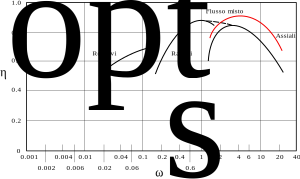
\includegraphics[width=.8\textwidth]{fig/PrestComp.pdf}
\caption{A destra le curve di rendimento per le macchine assiali. Si nota l'evidente aumento delle prestazioni (in rosso) rispetto alle prime macchine}
\label{fig:PrestComp}
\end{figure}
Nel diagramma in figura \ref{fig:PrestComp} è presente il rendimento del compressore in funzione della velocità specifica (che ricordiamo essere la caratteristica di macchina). Si nota che all'aumentare della velocità specifica si va verso macchine assiali, fino ad un certo punto della storia le macchine assiali non hanno goduto di rendimenti competitivi. In rosso è presentata la curva dello stato attuale dei rendimenti per macchine assiali. 
\begin{figure}
\centering
  \includegraphics[width=.5\textwidth]{fig/hsComp.png}
\caption{1: ingresso statore 2: uscita statore - entrata rotore 3: uscita statore.}
\label{fig:hsComp}
\end{figure}
Nel diagramma termodinamico in figura \ref{fig:hsComp} sono riportati gli stati di rierimento di uno stadio di compressore assiale. Nella parte rotorica avviene il lavoro con un relativo aumento della velocità mentre nello c'è il recupero in termini di pressione. Nello studio della macchina assiale vengono fatte generalmente le seguenti assunzioni:
\begin{itemize}
\item Flusso adiabatico;
\item Stadio ``normale" o ``ripetuto": tutti gli stadi hanno gli stessi profili
\begin{align*}
c_1 = c_2 \Rightarrow h_3-h_1 = h_{03} - h_{01}
\end{align*}
\item Velocità assiale costante (coincide con la velocità meridiana)
\begin{align*}
c_{m1} = c_{m2}
\end{align*}
\item densità costante nello stadio
\begin{align*}
\rho = cost. 
\end{align*}
\end{itemize}
\begin{align*}
\omega_s = \cfrac{\sqrt{\phi}}{\psi^{3/4}} \cdot \sqrt{\bigg( \cfrac{D_e}{D_i} \bigg)^2 -1}
\end{align*}
\begin{align*}
\phi = \frac{Q}{u \cdot S}
\end{align*}
\begin{align*}
\psi = \cfrac{\Delta h_{0is}}{\cfrac{u^2}{2}}
\end{align*}
\section{Lavoro e triangoli di velocità}
Nel rotore si conserva la rotalpia
\begin{equation}
h_1 + \frac{1}{2} w_1^2 = h_2 + \frac{1}{2} w_2^2
\end{equation}
Nello statore si conserva l'entalpia
\begin{equation}
h_2 + \frac{1}{2} c_2^2 = h_3 + \frac{1}{2} c_3^2
\end{equation}
Il lavoro scambiato è quello che avviene nella parte rotorica, definiamo un parametro adimensionale per quest'ultimo
\begin{equation}
\lambda = \frac{u \cdot c_{u2} - u \cdot c_{u1}}{u^2} = \frac{c_{u2} - c_{u1}}{u}
\end{equation}
\begin{figure}
\centering
  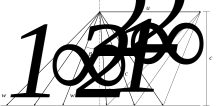
\includegraphics[width=.9\textwidth]{fig/triangComp.pdf}
\caption{}
\label{fig:triangComp}
\end{figure}
L'obiettivo è quello di determinare la relazione tra $\lambda$ e cifra di portata $\Phi$. Vado a disegnare i triangoli di velocità relativi allo stadio elementare come mostrato in figura \ref{fig:triangComp}. Ricordo che per definizione la componente meridiana e periferica sono costanti. Posso scrivere le seguenti tre relazioni 
\begin{align*}
c_{u2} = u - w_{u2}
\end{align*}
\begin{align*}
w_{u2} = c_m \tan \beta_2
\end{align*}
\begin{align*}
c_{u1} = c_m \tan \alpha_1
\end{align*}
Posso quindi scrivere
\begin{align*}
\lambda = 1- \frac{w_{u2}}{u} - \frac{c_{u1}}{u} = 1 - \frac{c_m}{u} \left(\tan \beta_2 + \tan \alpha_1 \right)
\end{align*}
Ma definendo  la cifra di portata come
\begin{align*}
\Phi = \frac{c_m}{u}
\end{align*}
Posso finalmente scrivere la cifra di flusso in funzione della cifra di portata, la caratteristica teorica del nostro compressore
\begin{equation}
\lambda = 1 - \Phi \left( \tan \beta_2 + \tan \alpha_1 \right) = 1 - k \cdot \Phi
\end{equation}
Con $k$ costante che dipende dalla geometria della macchina. Si tratta di una rappresentazione molto simile a quella nel caso delle pompe centrifuche nelle quali a seconda del valore di $k$ si ha la curva caratteristica della pompa; questo viene chiarito meglio dal diagramma in figura \ref{fig:CondProg}.
\begin{figure}
\centering
  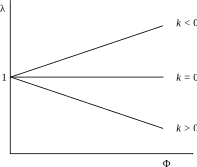
\includegraphics[width=.4\textwidth]{fig/CondProg.pdf}
\caption{}
\label{fig:CondProg}
\end{figure}
Andiamo ora a definire una condizione particolare di progetto ``lambda design"$\lambda_d$.
\begin{align*}
\lambda_d = 1 - k \cdot \Phi_d, \;\; k = f(\lambda_d,\Phi_d)
\end{align*}
Calcolo ora il rapporto $\lambda/\lambda_d$:
\begin{equation} \label{eq:lambdad}
\frac{\lambda}{\lambda_d} = \frac{1}{\lambda_d} - \frac{\Phi}{\Phi_d} \Bigg( \frac{1-\lambda_d}{\lambda_d} \Bigg), \;\;\; 0.3 < \lambda_d < 0.4
\end{equation}
Si tratta di una famiglia di rette, in figura \ref{fig:LambdaPhiChart} è rappresentato il diagramma caratteristico però in termini di rapporti rispetto alle condizioni di progetto. Si vede che nel caso ideale di $\lambda_d = 1$ il lavoro scambiato sarebbe indipendente dalla portata, sarebbe una situazione abbastanza attraente. 
\begin{figure}
\centering
\begin{minipage}{.5\textwidth}
  \centering
  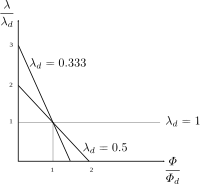
\includegraphics[width=.9\linewidth]{fig/LambdaPhiChart.pdf}
  \captionof{figure}{}
  \label{fig:LambdaPhiChart}
\end{minipage}%
\begin{minipage}{.5\textwidth}
  \centering
  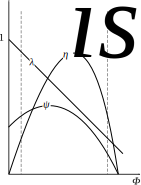
\includegraphics[width=.9\linewidth]{fig/CarattReal.pdf}
  \captionof{figure}{}
  \label{fig:CarattReal}
\end{minipage}
\end{figure}
Generalmente in un compressore, infatti, la pressione di output è definita mentre la portata è regolata, $\lambda_d = 1$ avrei una macchina perfetta, il rapporto di pressione lo riuscirei sempre a mantenere e basta che regoli la portata per ottenere la pressione voluta. Purtroppo non è così perchè le palettature non si comportano in modo ideale, si hanno separazioni di vela, inspessimenti di strato limite... dal punto di vista realistico si riesce ad ottenere un $\lambda_d$ definito come nell'equazione \ref{eq:lambdad}. 

Come mostrato in figura \ref{fig:CarattReal} otterrò un comportamento non ideale che non avrà andament rettilineo, avrtò quindi un campo di utilizzo essendo limitato sia a portate basse che a portate alte. 

Caratteristica reale:
\begin{equation}
\psi = \frac{\Delta h_{0is}}{u^2} = \lambda \cdot \eta_{is}, \;\;\; \Delta h_{0is} = h_{30is} - h_{10}
\end{equation}

Non abbiamo ancora detto nulla riguardo la forma della pala in funzione del grado di reazione\footnote{Che ricordiamo essere il rapporto tra il salto entalpico elaborato tra parte rotorica e statorica}. 
\begin{align*}
R = \frac{h_2 - h_1}{h_3-h_1} 
\end{align*}
Sapendo che
\begin{align*}
\begin{rcases*}
c_{u2} = u - w_{u2}\\
c_{u1} = u - w_{u1}
\end{rcases*}
\Rightarrow c_{u2} - c_{u1} = w_{u1} - w_{u2} 
\end{align*}
Vado a sviluppare il grado di reazione della macchina applicando la conservazione della rotalpia al numeratore e l'espressione del lavoro euleriano al denominatore:
\begin{align*}
R = \frac{w_1^2 - w_2^2}{2 u (c_{u2} - c_{u1})} &= \frac{(w_{u1} + w_{u2})\cancel{(w_{u1}-w_{u2})}}{2 u \cancel{(c_{u2} - c_{u1})}} =\\
&= \frac{w_{u1} + w_{u2}}{2u} = \\
&= \frac{c_m \left(\tan \beta_1 + \tan \beta_2 \right)}{2 u}
\end{align*}
Definendo poi
\begin{align*}
\tan \beta_{\infty} = \frac{\tan \beta_1 + \tan \beta_2}{2}, \;\; \Phi = \frac{c_m}{u}
\end{align*}
Si ottiene
\begin{equation}
\boxed{R = \Phi \tan \beta_{\infty} = \frac{w_{u \infty}}{u}}
\end{equation}
Lo stesso risultato poteva essere raggiunto nel seguente modo
\begin{equation}
w_{u1} = u - c_{u1} \; \Rightarrow \; R = \frac{1}{2} + \frac{\tan \beta_2 - \tan \alpha_1}{2} \cdot \Phi \simeq \frac{1}{2} + cost \cdot \Phi
\end{equation}
Quello che è importante notare è che:
\begin{align*}
R = 0.5 \to \beta_2 = \alpha_1
\end{align*}
Il grado di reazione è costante con la portata e la palettatura sarà simmetrica.

Per rappresentare lo stadio al variare del grado di reazione andiamo per prima cosa a definire i triangoli di velocità come si vede in figura \ref{fig:StadioRipetuto}.
\begin{figure}
\centering
  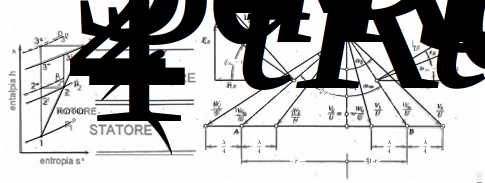
\includegraphics[width=\textwidth]{fig/StadioRipetuto.pdf}
\caption{}
\label{fig:StadioRipetuto}
\end{figure}
Sempre facendo riferimento alla figura posso quindi scrivere
\begin{align*}
r \cdot \tan \beta_{\infty} = R 
\end{align*}
\begin{align*}
\lambda = \cfrac{\Delta h_0}{\cfrac{u^2}{2}} = \cfrac{u \Delta c_u}{\cfrac{u^2}{2}} = \cfrac{2 \Delta c_u}{u} = \cfrac{2 \Delta w_u}{u}
\end{align*}
\begin{align*}
\frac{\Delta c_u}{u} = \frac{\Delta w_u}{u} = \frac{\lambda}{2}
\end{align*}
Qual'ora si operi un cambio di portata vediamo che gli unici angoli che si conservano sono $\beta_2$ e $\alpha_1$, la cifra si flusso passa dalle condizioni di design $\Phi_d$ alle condizioni generiche $\Phi$ come si vede in figura \ref{fig:CondFuoriProg}.
\begin{figure}
\centering
  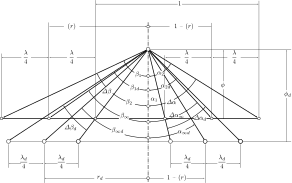
\includegraphics[width=\textwidth]{fig/CondFuoriProg.pdf}
\caption{}
\label{fig:CondFuoriProg}
\end{figure}

Possiamo classificare alcune condizioni notevoli riportate in figura \ref{fig:ComprAssTab}.
\begin{figure}
\centering
  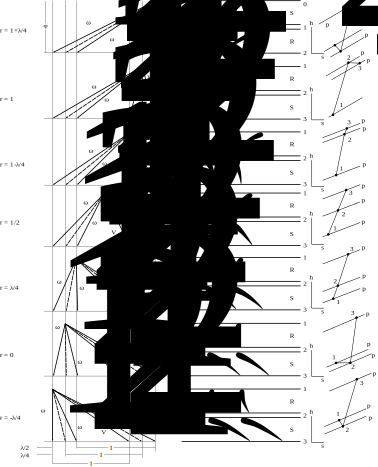
\includegraphics[width=1.2\textwidth]{fig/ComprAssTab.pdf}
\caption{}
\label{fig:ComprAssTab}
\end{figure}
Il primo caso con $r = 1 + \lambda /4$ è particolare in quanto si ha grado di reazione maggiore di uno, lo statore precede infatti il rotore. Mi ritrovo con una velocità di uscita puramente assiale.

Con grado di reazione $r = 1$ le velocità assolute ingresso uscita sono simmetriche.

Con $r = 1 - \lambda/4$ la velocità assoluta è puramente assiale, mentre quella allo scarico non lo è. 

Sono poi rappresentate le geometrie per gradi di reazione sempre più ridotti. 

La soluzione $r = 1/2$ è la più diffusa e utilizzata eccetto per il primo e l'ultimo stadio in cui si vogliono distribuzioni di velocità particolari, velicità assoluta in uscita e poi in ingresso puramente assiale. In questa configurazione si avranno profili uguali ma specchiati, l'intervallo p1 p3 è poi diviso equamente in due parti uguali tra la parte statorica e la parte rotorica. 

\section{Termodinamica}
Vediamo il calcolo del rendimento al variare della portata e del grado di reazione. Partiamo dalla definizione di rendimento isoentropico
\begin{align*}
\eta_{is} = \frac{\Delta h_{is}}{\Delta h_0} = \frac{\Delta p}{\rho \cdot \Delta h_0}
\end{align*}
Dal primo principio:
\begin{align*}
T ds = dh - \frac{dp}{\rho}
\end{align*}
ma
\begin{align*}
ds = 0 \Rightarrow dh = \frac{dp}{\rho}
\end{align*}
Otteniamo quindi
\begin{equation}\label{eq:etadp}
\eta_{is} = \frac{\Delta p}{\rho \cdot \Delta h_0} = \cfrac{\Delta p}{\rho \cdot \cfrac{\lambda}{2} u^2}
\end{equation}
L'incremento di pressione totale si può però ulteriormente sviluppare come somma di incremento di pressione sviluppato nel rotore e nello statore
\begin{align*}
\Delta p = \Delta p_R + \Delta p_S = \frac{F_{aR}}{s_R} + \frac{F_{aS}}{s_S} = \frac{F_{tR} \cdot \tan(\beta_{\infty} - \varepsilon_R)}{s_R} + \frac{F_{tS} \cdot \tan(\alpha_{\infty} - \varepsilon_S)}{s_S}
\end{align*}
Con $\varepsilon_S, \; \varepsilon_R$\footnote{Per quanto riguarda i pedici "s" sta per statore, "r" per rotore.} indice di efficienza del profilo.
Possiamo fare qualche assunzione. I profili hanno drag molto più piccolo del lift quindi
\begin{align*}
\tan \varepsilon_R \simeq \varepsilon_R = \frac{D_R}{L_R} \;\;\;\;\; \tan \varepsilon_S \simeq \varepsilon_S = \frac{D_S}{L_S}
\end{align*}
Utilizzando le componenti di forza del triangolo di velocità si ottiene
\begin{align*}
F_{tR} = \dot{m} \Delta w_u = \overbrace{s_R \cdot \rho \cdot c_m}^\text{$ \dot{m} $} \cdot \overbrace{\lambda \cdot u \cdot \frac{1}{2}}^\text{$\Delta w_u$}  
\end{align*}
Analogamente riesco a fare la stessa cosa per la parte statorica
\begin{align*}
F_{tS} = \dot{m} \Delta c_m = s_S \cdot \rho \cdot \lambda \cdot \Phi \cdot u^2 \cdot \frac{1}{2}
\end{align*}
Andando a sostituire
\begin{align*}
\Delta p = \frac{1}{2} \rho \lambda u^2 \big[ \Phi \tan \left( \beta_{\infty} - \varepsilon_R \right) + \Phi \tan \left( \alpha_{\infty} - \varepsilon_S \right) \big] 
\end{align*}
Ricordando le relazioni
\begin{align*}
R = \Phi \tan \beta_{\infty}
\end{align*}
\begin{align*}
1 - R = \Phi \tan \alpha_{\infty} 
\end{align*}
\begin{align*}
\tan ( \beta_{\infty} - \varepsilon_R ) = \frac{\tan \beta_{\infty} - \tan \varepsilon_R}{1 + \tan \beta_{\infty} \tan \varepsilon_R} \simeq \frac{\tan \beta_{\infty} - \varepsilon_R}{1 + \tan \beta_{\infty} \cdot \varepsilon_R}
\end{align*}
\begin{align*}
\tan (\alpha_{\infty} - \varepsilon_S) \simeq \frac{\tan \alpha_{\infty} - \varepsilon_S}{1 + \tan \alpha_{\infty} \cdot \epsilon_S}
\end{align*}
Ottengo in fine la relazione del salto di pressione in funzione del grado di reazione e di $\lambda$:
\begin{equation}
\Delta p = \frac{1}{2} \rho \lambda u^2 \Bigg[ \frac{R - \varepsilon_R \Phi}{\Phi + \varepsilon_R R} + \frac{1 - R - \varepsilon_S \Phi}{\Phi + \varepsilon_S (1-R)} \Bigg] \cdot \Phi
\end{equation}
Posso dire che epsilon r è circa epsilon s. Il rendimento isoentropico ricordando l'equazione \ref{eq:etadp} diviene:
\begin{equation}
\boxed{ \eta_{is} = \Bigg[ \frac{R - \varepsilon_R \Phi}{\Phi + \varepsilon_R R} + \frac{1 - R - \varepsilon_S \Phi}{\Phi + \varepsilon_S (1-R)} \Bigg] \cdot \Phi }
\end{equation}
Cerco ora il coefficiente di reazione
\begin{align*}
\varepsilon_S \simeq \varepsilon_R = cost = \varepsilon
\end{align*}
\begin{align*}
\frac{d \eta_{is}}{dR} = 0 \Rightarrow R_{opt} = 0.5 per \forall \Phi
\end{align*}
\begin{align*}
\eta_{|R= 0.5} = 2 \Phi \cdot \frac{1- 2 \varepsilon \Phi}{\varepsilon + 2 \Phi}
\end{align*}
Si ha quindi $R_{opt} = 0.5$. 
Naturalmente si vede che il rendimento del compressore è migliorato alla diminuzione di $\varepsilon$.
\begin{align*}
\frac{d\eta_{|R=0.5}}{d \Phi} = 0 \Rightarrow \Phi_{opt} = \frac{1}{2} \left( \sqrt{1 + \varepsilon^2} - \varepsilon \right) \simeq \frac{1 - \varepsilon}{2}
\end{align*}
Determino ora il rendimento ottimale in funzione di $\Phi$
\begin{equation}
\eta_{max} = 1 + 2 \varepsilon^2 - 2 \varepsilon \sqrt{1 + \varepsilon^2} \simeq 1 - 2 \varepsilon \left( 1 - \varepsilon \right)
\end{equation}
\begin{figure}
\centering
  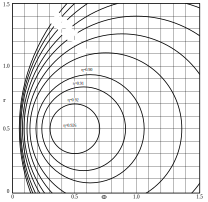
\includegraphics[width=\textwidth]{fig/IsoRendCompAss.pdf}
\caption{Curve isorendimento di uno stadio assiale in funzione del grado di reazione e coefficiente di portata per efficienza del profilo assegnata}
\label{}
\end{figure}

\section{Progettazione della schiera}
\subsection{Correlazioni di Howell}
Sono presenti molteplici correlazioni per progettare una macchina assiale. Noi vedremo un filone di correlazioni, sono datate ma non hanno perso di validità. Anche nella progettazione di una nuova macchina è utile partire da un predimensionamento per poi andare a raffinare con strumenti moderni. Verrà quindi usato come passo preliminare.
Si parte dalle seguenti riflessioni:
\begin{itemize}
\item La deflessione imposta alla corrente è limitata: nell'ordine delle decine di gradi (20, 30 al massimo 40);
\item Profili sottili a bassa curvatura.
\end{itemize}
Le perdite possono quindi essere suddivise in 
\begin{itemize}
\item Perdite di anello;
\item perdite di profilo;
\item perdite per flussi secondari.
\end{itemize}
La perdita di profilo è direttamente correlata al $c_D$, sarà quella in cui si può andare maggiormente a lavorare. 
Il flusso all'interno del compressore è un moto elicoidale. Il flusso lambisce la cassa della macchina, vi sarà quindi un attrito tra fluido e la partete, queste perdite le chiameremo perdite di ``anello".
Le perdite per flussi secondari sono state adeguatamente trattate nel capitolo precedente. 
Si andrà quindi a lavorare sulle perdite di profilo aggiungendo poi le altre due perdite tramite coefficienti di correlazione.

Le perdite di anello inducono un drag aggiuntivo correlato a quanto più è elevato lo sviluppo radiale della pala, definito $H$ lo sviluppo radiale e $s$ passo palare, si può scrivere
\begin{align*}
C_{Da} = 0.02 \cdot \frac{s}{H}
\end{align*}
Abbiamo poi che la perdita per flussi secondari è correlata con il quadrato del coefficiente di portanza, quanto più io ho una portanza elevata quanto più impongo una deviazione, tanto più è probabile che abbia un instaurarsi di moti secondari.
\begin{align*}
C_{Da} = 0.018 \cdot C_L^2
\end{align*}
Posso andare quindi a scrivere un coefficiente di resistenza complessivo
\begin{align*}
C_{Dtot} = C_D + C_{Da} + C_{Ds} = C_D + 0.02 \cdot \frac{s}{H} + 0.018 \cdot C_L^2
\end{align*}
In figura \ref{fig:ComprStageLoss} si vede come le varie perdite inficiano sull'efficienza della schiera.
\begin{figure}
\centering
  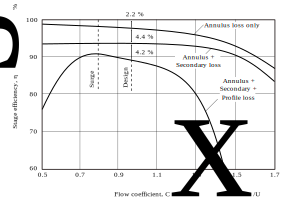
\includegraphics[width=\textwidth]{fig/ComprStageLoss.pdf}
\caption{}
\label{fig:ComprStageLoss}
\end{figure}
La progettazione preliminare con la correlazione di Howell, si va a cercare la relazione tra gli angoli geometrici in ingresso e uscita e gli angoli che deve avere il fluido. La prima correlazione di Howell dice che la condizione di riferimento, ovvero la deflessione che la corrente subisce nell'attraversamento delle pale (nominale) $\varepsilon^*$ viene riferita rispetto alla deviazione di stallo $\varepsilon_s$
\begin{equation}
\varepsilon^* = 0.8 \cdot \varepsilon_s
\end{equation}
In figura \ref{fig:Howell} è rappresentato l'andamento della deflessione in funzione dell'angolo di incidenza. Come si nota un tratto pressocchè lineare seguito da un brusco cambiamento di curvatura. Quest'ultimo è facilmente individuabile, risutlta quindi comodo utilizzarlo come punto di riferimento per individuare la deflessione nominale. Cpme deflessione nominale si utilizzarà quindi un valore che va a minimizzare le perdite, tenendo conto poi dei margini di operabilità.  
\begin{figure}
\centering
  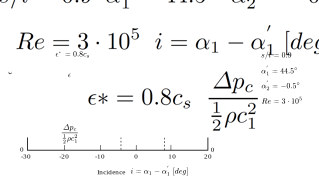
\includegraphics[width=\textwidth]{fig/Howell.pdf}
\caption{}
\label{fig:Howell}
\end{figure}
In figura \ref{fig:SchieraDim} si riportano le nomenclature utilizzate in questo capitolo, è rappresentata la differenza tra angoli geometrici e fluidodinamici.
\begin{figure}
\centering
  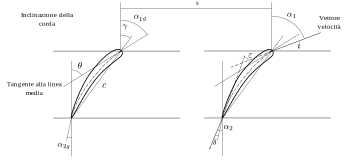
\includegraphics[width=\textwidth]{fig/SchieraDim.pdf}
\caption{}
\label{fig:SchieraDim}
\end{figure}
La prima correlazione di Howell permette di calcolare gli angoli del flusso attesi da una chiera di data solidità ($\varepsilon = \varepsilon*$).
La seconda correlazione di Howell permette di trovare, noti gli angoli di flusso, i corrispondenti valori degli angoli geometrici della schiera ($\varepsilon = \varepsilon*$).
La terza correlazione di Howell permette di calcolare le prestazioni in off-design, quando $\varepsilon \neq \varepsilon*$ 
In figura \ref{fig:1CorrHowell} è rappresentata la prima correlazione di Howell al variare della solidità della schiera. Si nota che a parità di deflessine nominalre si avrà una maggiore angolo in uscira per schiere più compatte.
\begin{figure}
\centering
  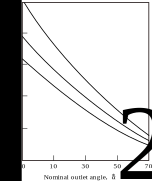
\includegraphics[width=.4\textwidth]{fig/1CorrHowell.pdf}
\caption{}
\label{fig:1CorrHowell}
\end{figure}
Si definisce il campo di validità della relazione
\begin{align*}
\varepsilon^* = f \bigg( \frac{s}{l}, \alpha_2^*, Re \bigg) \;\; 20^{\circ} < \theta < 40^{\circ}
\end{align*}
\begin{align*}
\varepsilon^* = f\bigg(\frac{s}{l}, \alpha_2*\bigg)\;\; Re > 3 \cdot 10^5
\end{align*}
La deflessione nominale è definita come segue
\begin{align*}
\varepsilon^* = \alpha_1^* - \alpha_2^*
\end{align*}
Le curve espresse come relazione tra gli angoli
\begin{align*}
\tan \alpha_1^* - \tan \alpha_2^* = \cfrac{1.55}{1 + 1.5 \cfrac{s}{l}}
\end{align*}
La seconda correlazione di Howell mi da il valore della deviazione $\delta$, lo scostamento tra angolo geometrico e angolo effettivo del flusso in uscita. Si ha che $\delta$ dipende dai seguenti fattori
\begin{align*}
\delta = f \bigg( \theta, forma \; della \; pala, \frac{s}{l}, \gamma \bigg)
\end{align*}
Si usa la seguente relazione
\begin{align*}
\delta^* = m \theta \bigg( \frac{s}{l} \bigg)^n
\end{align*}
con $n = 1/2$ per schiere di compressore e $n = 1$ per schiere di IGV. Il coefficiente $m$ è funzione della forma della pala, si ripete che queste sono correlazioni approssimative.
\begin{align*}
m = 0.23 \cdot \bigg( 2 \cdot \frac{a}{l} \bigg)^2 + \frac{\alpha_2^*}{500}
\end{align*}
Con queste correlazioni posso ridurre i gradi di libertà nella definizione della geometria. Infatti una volta scelti $ \theta, \sigma $, dalla seconda correlazione ottengo $ \delta^* $ e dalla prima corrlazione trovo $ \varepsilon^* $. In questo modo posso definire
\begin{align*}
i^* = \varepsilon^* - \theta + \delta^*
\end{align*}
\begin{align*}
\alpha_{1g} = \alpha_1^* - i^*
\end{align*}
\begin{align*}
\alpha_{1g} = \alpha_2^* - \delta^*
\end{align*}
Ora posso effettivamente disegnare la schiera. 

\subsection{Condizioni fuori progetto}
Si utilizzano delle ulteriori relazioni nelle quali si va a rapportare la deflessione relativa $\varepsilon/\varepsilon^*$ rispetto alle altre caratteristiche (figura \ref{fig:FuoriProg1})
\begin{figure}
\centering
  \includegraphics[width=\textwidth]{fig/FuoriProg1.pdf}
\caption{}
\label{fig:FuoriProg1}
\end{figure}
Queste relazioni sono state ricavati per numeri di Mach bassi, vediamo cosa succede aumentando la velocità e quindi avvicinandosi alle condizioni soniche. In figura \ref{fig:FuoriProg2} si rapporta il coefficiente di pressione In il numero di Mach in entrata. 
\begin{figure}
\centering
\begin{minipage}{.6\textwidth}
  \centering
  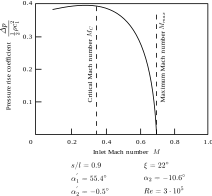
\includegraphics[width=.95\linewidth]{fig/FuoriProg2.pdf}
  \captionof{figure}{}
  \label{fig:FuoriProg2}
\end{minipage}%
\begin{minipage}{.4\textwidth}
  \centering
  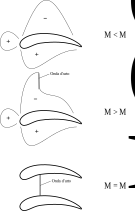
\includegraphics[width=.95\linewidth]{fig/FuoriProgMach.pdf}
  \captionof{figure}{ Campo di pressione attorno al profilo al variare del numero di Mach}
  \label{fig:FuoriProgMach}
\end{minipage}
\end{figure}
Il diagramma è riferito a condizioni specifiche. Di divide la curva in due parti da $M_C$, oltre questo Mach critico l'andamento delle pressioni sul singolo profilo, Fintanto che $ M < M_C$ l'andamento è quello mostrato in figura. Al crescere di $M$ il campo di pressione attorno al profilo si modifica con la possibile formazione di un'onda d'urto, il recupero di pressione varia anch'esso in maniera sensibile perggiorando le prestazioni del profilo. Nella condizione di $ M_{max} $ si ha un'onda d'urto che occupa l'intero condotto, sono in chocking e la portata non può variare.
\begin{figure}
\centering
  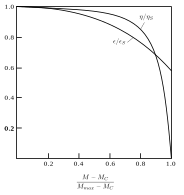
\includegraphics[width=.4\textwidth]{fig/FuoriProg3.pdf}
\caption{}
\label{fig:FuoriProg3}
\end{figure}
In figura \ref{fig:FuoriProg3} ho le relazioni che mi correlano deflessione della schiera e rendimento in funzione di una grandezza dipendente da $M$ completamente definita una volta definiti $M_C$ e $M_{max}$ che ricordiamo essere specifici per condizioni fissate; soprattutto $M_C$ è pesantemente influenzato dall'angolo di incidenza come si vede in figura \ref{fig:FuoriProg4}.
\begin{figure}
\centering
  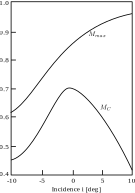
\includegraphics[width=.4\textwidth]{fig/FuoriProg4.pdf}
\caption{}
\label{fig:FuoriProg4}
\end{figure}

\subsection{Criterio di carico}
Al variare del numero di pale, a parità di lavoro svolto dalla macchina dovrò imporre diverse deflessioni, ne conseguirà un carico diverso sulla singola pala. Con poche pale dovrò infatti imporre deflessioni maggiori con un forte carico sul singolo profilo.
Si va a fare una verifica, fissata la schiera e la solidità si va a calcolare il coefficiente di deflessione locale $D_{loc}$ che dice quant'è la massima decelerazione a cui è soggetta la schiera (eq. \ref{eq:D_loc}). Si considera poi la riduzione di quantità di moto come nell'equazione \ref{eq:D_ridqmot} integrando sullo spessore occupato dalla scia, con $V$ è velocità di riferimento mentre $\nu$ è la velocità come funzione della posizione.
\begin{figure}
\centering
  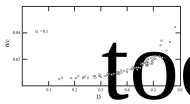
\includegraphics[width=\textwidth]{fig/CritCarico1.pdf}
\caption{}
\label{fig:CritCarico1}
\end{figure}
Fattore di diffusione locale
\begin{equation}\label{eq:D_loc}
D_{loc} = \frac{V_{max} - V_2}{V_{max}}
\end{equation}
\begin{equation}\label{eq:D_ridqmot}
\theta = \int_{\delta_P}^{\delta_S} \frac{\nu}{V} \bigg(1- \frac{\nu}{V} \bigg) dy
\end{equation} 
\begin{figure}
\centering
  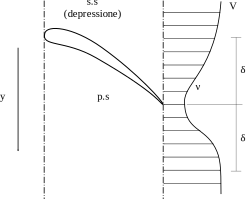
\includegraphics[width=.4\textwidth]{fig/CritCarico2.pdf}
\caption{}
\label{fig:CritCarico2}
\end{figure}
Se ho molte pale, l'integrale diventa molto grande perchè potrei avere l'intero canale palare occupato dalla scia, quindi come criterio empirico utilizzo
\begin{align*}
\frac{\theta}{c} < 0.2
\end{align*}
In questo modo l'inspessimento di strato limite è considerato trascurabile rispetto alla corrente principale. 
\begin{figure}
\centering
  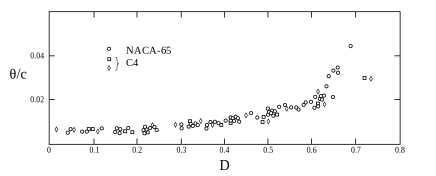
\includegraphics[width=\textwidth]{fig/CritCarico3.pdf}
\caption{}
\label{fig:CritCarico3}
\end{figure}
Il valore di $D$ si può calcolare anche attraverso differenti correlazioni (figura \ref{fig:CritCarico3})
\begin{align*}
D = \bigg( \frac{V_1 - V_2}{V_1} \bigg) + \bigg( \frac{V_{t1} - V_{t2}}{2 \sigma V_1} \bigg) = \bigg( 1 - \frac{\cos \alpha_1}{cos \alpha_2} \bigg) + \frac{\cos \alpha_1}{2 \sigma} (\tan \alpha_1 - \tan \alpha_2)
\end{align*}
e come criterio empirico si usa $$ D \leqslant 0.4 \div 0.5  $$
\begin{figure}
\centering
  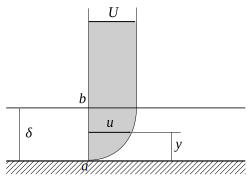
\includegraphics[width=.4\textwidth]{fig/CritCarico4.pdf}
\caption{}
\label{fig:CritCarico4}
\end{figure}
Infine si possono andare a cercare correlazioni rispetto allo strato limite come mostrato in figura \ref{fig:CritCarico4} ma ciò non ha molto senso in quanto nel contesto moderno è propio la parte di progettazione che si effettua per via numerica. 
\begin{align*}
\Delta M = \int_0^{\delta} \rho u dy (U-u) = \rho \int_0^{\delta} u (U-u) dy
\end{align*} 
Spessore della quantità di moto dello strato limite
\begin{equation}
\theta = \frac{\Delta M}{\rho U^2} = \int_0^{\delta} \frac{u}{U} \bigg( 1 -\frac{u}{U} \bigg) dy
\end{equation}

\section{Schiere supersoniche}
Fin'ora abbiamo parlato di schiere di copressori con deflusso subsonico debolmente comprimibile con rapporti di compressione modesti (10 - 20 peerc) partendo dal presupposto che il flusso in ingresso sia inferiore alla velocità sonica. Quindi 
\begin{align*}
\begin{cases}
M_1 <1\\
M_2 <1
\end{cases}
\end{align*} 
Vediamo delle condizioni diverse. Si parlerà di compressore transonico se 
\begin{align*}
\begin{cases}
M_1 >1\\
M_2 <1
\end{cases}
\end{align*} 
Nel caso in cui si arrivi in condizione soniche all'interno della macchina si faranno ulteriori distinzioni rispetto alla componente assiale: per $M_{1a} < 1 $ si parlerà di \textit{regime innescato} o \textit{non innescato} mentre per $ M_{1a} > 1 $ si parlerà di \textit{regime saturo}.
Ulteriori possibilità che non hanno però rilevanza nei compressori sono 
\begin{align*}
\begin{cases}
M_1 <1\\
M_2 >1
\end{cases}
\end{align*} 
In questo caso il flusso viene accelerato ma per definizione in un compressore cerco esattamente l'effetto opposto. Si ha poi
\begin{align*}
\begin{cases}
M_1 >1\\
M_2 >1
\end{cases}
\end{align*} 
in cui il flusso è interamente supersonico, non ha interessi applicativi.

Le schiere supersoniche trovano applicazioni particolari in campo aeronautico. Nel regime non innescato notiamo che è presente un'onda d'urto normale al flusso, si avrà una zona supersonica a monte della schiera, l'aumento di velocità naturalmente è dovuto all'aumento di spessore della schiera.

Nel regime innescato la perturbazione di pressione occupa integralmente il condoto palare, distinguo in maniera chiara, la portata è bloccata. 

In regime saturo la componente assiale è superiore a 1, il blocco sonico è a monte della schiera, a monte si creano onde oblique che dissipano energia.

\begin{figure}[h!]
\centering
  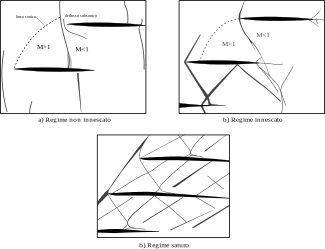
\includegraphics[width=.8\textwidth]{fig/Schlieren1.pdf}
\caption{}
\label{fig:Schlieren1}
\end{figure}
\begin{figure}[h!]
\centering
  \includegraphics[width=.8\textwidth]{fig/Schlieren2.png}
\caption{}
\label{fig:Schlieren2}
\end{figure}
Questo tipo di deflusso consente un salto di pressione più elevato a scapito però di una pesante perdita in termini di rendimento. 
